% This is samplepaper.tex, a sample chapter demonstrating the
% LLNCS macro package for Springer Computer Science proceedings;
% Version 2.20 of 2017/10/04
%
\documentclass[runningheads]{llncs}
%
\usepackage{graphicx}
\usepackage{syntax}
\usepackage{listings}
\usepackage{listings-rust}
\usepackage{listings-golang}
\usepackage{amsmath}
\usepackage[section]{placeins}
\titlerunning{Christopher Henderson \and Ajay Bansal}

% Better inline directory listings
% \usepackage{xcolor}
% \definecolor{light-gray}{gray}{0.95}
% \newcommand{\code}[1]{\colorbox{light-gray}{\texttt{#1}}
\newcommand{\code}[1]{\texttt{#1}}
% Used for displaying a sample figure. If possible, figure files should
% be included in EPS format.
%
% If you use the hyperref package, please uncomment the following line
% to display URLs in blue roman font according to Springer's eBook style:
% \renewcommand\UrlFont{\color{blue}\rmfamily}

\begin{document}
%
\title{Declarative Search Construct in Imperative/Procedural Programming Languages}
%
%\titlerunning{Abbreviated paper title}
% If the paper title is too long for the running head, you can set
% an abbreviated paper title here
%
\author{Christopher Henderson\inst{1} \and Ajay Bansal\inst{1}}
% First names are abbreviated in the running head.
% If there are more than two authors, 'et al.' is used.
%
\institute{Arizona State University, Tempe AZ 85281, USA
\url{https://www.asu.edu}
}
%
\maketitle              % typeset the header of the contribution
%
\begin{abstract}
Graph theory is a critical component of computer science and software engineering, with algorithms concerning graph traversal and comprehension powering much of the complex problems in both industry and research. Engineers and researchers often have an accurate view of their target graph, however they struggle to implement a correct, and efficient, search over that graph. Even though modern imperative languages provide libraries for graph search, there are no built-in constructs for search with separation of concerns, that is separate the implementation of graph traversal from the user’s desired search result. In this paper, we propose a new programming language construct, the search statement, in order to facilitate rapid, correct, efficient, and intuitive development of graph-based solutions. Given a supra-root node, a procedure which determines the children of a given parent node, and optional definitions of the fail-fast acceptance or rejection of a solution, the search statement can conduct a search over any graph or network. Structurally, this statement is modeled after the common switch statement and is put into a largely imperative/procedural context to allow for declarative and intuitive development by most programmers. The Go programming language has been used as a foundation and proof-of-concept of the search statement. 

\keywords 
{
Backtracking \and
Graph Search \and
Imperative Programming \and
Declarative Programming
}

\end{abstract}
\addtocontents{toc}{\setcounter{tocdepth}{5}}

\tableofcontents
\listoffigures
\listoftables
\newpage

\section{Introduction}
This paper will attempt to bring a component often associated with declarative programming, automated graph search as a first class citizen, into an imperative/procedural context. We will explore the \code{search} construct which, at least aesthetically, appears much like the traditional \code{switch} statement found in many popular programming language.

\begin{figure}
\begin{lstlisting}[language=golang, style=boxed]
search FCG {
	children:
		...
	reject:
		...
	accept:
		...
}
\end{lstlisting}
\end{figure}

\section{Background}

\section{Methodology}
.....embed the \code{search} construct within an already working, well known, programming language in order to facilitate observations about its interactions with 

\section{Related Work}
Prolog's proof search.

\begin{figure}
\begin{lstlisting}[language=Prolog]
f(a). 
f(b).
g(a). 
g(b).
h(b).
k(X) :- f(X), g(X), h(X).
\end{lstlisting}
\caption{Given k(X), Prolog will succeed in unifying f(a) and g(a) but fail to unify h(a). Prolog will then bactrack and attempt to unify f(b), g(b), and h(b) which all succeed, thus unifying X with b}
\end{figure}
% /////////

\begin{figure}
\begin{quotation}
In order to apply backtracking to a specific class of problems, one must provide the data P for the particular instance of the problem that is to be solved, and six procedural parameters, root, reject, accept, first, next, and output. These procedures should take the instance data P as a parameter and should do the following:
1. root(P): return the partial candidate at the root of the search tree.
2. reject(P,c): return true only if the partial candidate c is not worth completing.
3. accept(P,c): return true if c is a solution of P, and false otherwise.
4. first(P,c): generate the first extension of candidate c.
5. next(P,s): generate the next alternative extension of a candidate, after the extension s.
6. output(P,c): use the solution c of P, as appropriate to the application.
The backtracking algorithm reduces the problem to the call bt(root(P)), where bt is the following recursive procedure:
\begin{lstlisting}[escapeinside={(*}{*)}]
procedure bt(c)
	if reject(P,c) then return
	if accept(P,c) then output(P,c)
	s ← first(P,c)
	whiles (*$\neq$*) (*$\wedge$*) do bt(s)
		s (*$\leftarrow$*) next(P,s)
\end{lstlisting}
\caption{Operational semantics of backtracking.\cite{wikipediaBacktrack}}
\end{quotation}
\end{figure}

\section{Our Approach}
Build a compiler based off of THE most C like modern language

\subsection{The \code{search} statement}

\subsection{The First Choice Generator}
Every graph has, external to the universe of the graph itself, a node which selects all of the
possible first choices of that graph. It is the node from which no choices have yet been made. We will call this node the First Choice Generator (FCG). The FCG is not a member of the graph itself nor will it ever be a member of the solution to a particular search. The FCG acts solely as an oracle which informs the algorithm of all possible starting points for a given search. The definition of the FCG and its graphs is the following recurrence relationship:

\begin{figure}
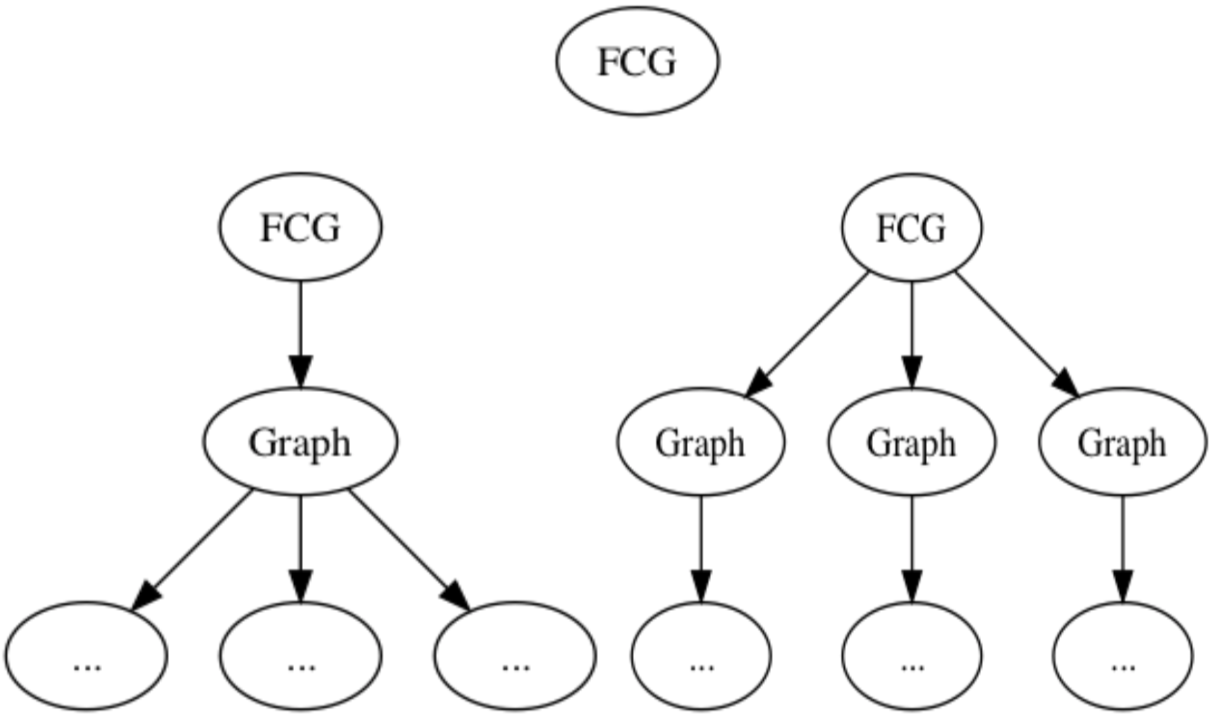
\includegraphics[width=\textwidth]{images/fcg.png}
\title{The First Choice Generator}
\label{The First Choice Generator}
\caption{An FCG followed by no graph. An FCG followed by a single graph. An FCG followed by multiple graphs.}
\end{figure}

\begin{equation}
  FCG=\begin{cases}
  	& \text{An FCG}.\\
  	& \text{An FCG followed by one or more graphs}.
  	\end{cases}
\end{equation}

\begin{equation}
  Graph=\begin{cases}
  	& \text{A node}.\\
  	& \text{A node followed by one or more graphs}.
  	\end{cases}
\end{equation}

The distinction between the two relationships, specifically the distinction between the FCG and a regular node, is that the FCG is not considered to be a member for the graph. Rather, it advises on how to begin the search.

Every search begins at an FCG, as it advises on how to begin the search. Future ellision rules may be discovered and implemented if an FCG with exactly one child proves to be the most common scenario and such a case is detectable by a compiler.

\subsection{\code{search} signature}

The signature of the search construct appears superficially similar to that of the \code{switch} statement seen in many programming languages. It consists of the word \code{switch} followed by an expression which evaluates to a valid FCG.

\subsection{\code{children}}
Given a procedure which accepts a node and returns a list of nodes, a graph may be traversed in any arbitrary fashion. The \code{children} procedure consults the graph search on how to procede forward from any given node from within the graph. The order in which the user provided procedure produces its children guides the underlying engine on how to traverse the graph, although current implementations mandate the use of a depth-firs search (DFS) strategy from within the engine. The choice of a DFS implementation is irrespective as future implementations can just as opaquely provide dispatch to alternative search strategies. The \code{children} block is defined as follows:
\\
\\
\textit{The \code{children} procedure accepts a node and returns a list of nodes. Optionally, the \code{children} procedure may additionally be provided with a list of nodes representing the solution computed thus far, thus facilitating algorithms which make their decisions via heuristics.}

\begin{figure}
\begin{lstlisting}
children(parent Node[, solution [Node]]) -> [Node]
\end{lstlisting}
\caption{Signature of the \code{children} procedure.}
\end{figure}

\subsection{\code{reject}}

\textit{The \code{reject} procedure accepts a candidate member node of a solution and a list of nodes representing the solution computed thus far, and returns a boolean value indicating whether or not that candidate node represents a dead-end in the computation.}

Given the above definitiona a graph search can be conducted in a \textit{fail fast} fashion. This facilitates algorithms such as bactracking.


\begin{figure}
\begin{lstlisting}
reject(candidate Node, solution [Node]) -> bool
\end{lstlisting}
\caption{Signature of the \code{reject} procedure.}
\end{figure}


\subsection{\code{accept}}

\textit{The \code{accept} procedure accepts a list of nodes representing the solution computed thus far and returns a boolean value indicating whether or not the solution in question is a whole, complete, and correct solution to the current problem.}

\begin{figure}
\begin{lstlisting}[xleftmargin=.2\textwidth]
accept(solution [Node]) -> bool
\end{lstlisting}
\caption{Signature of the \code{accept} procedure.}
\end{figure}

\subsection{Engine Psuedo Code Implementation}
The following is a psuedo code implementation of the \code{search} engine as a recursive, higher order, procedure. Brackets within the signature and procedure body indicate optional parameters and code paths.

See Appendix A and Appendix B for implementations in the Go and Rust programming languages whose most notable difference is manual management of a stack that is allocated to the free store, thus avoiding the risk of stack overflow errors.

\begin{lstlisting}[escapeinside={(*}{*)}]
let procedure search(FCG, solution[, accept, reject]):
	[if reject(FCG, solution):
		return]
	[if accept(solution):
		return]
	for child (*$\in$*) children(root):
		search(child, solution[, accept, reject])
\end{lstlisting}

\subsection{EBNF Grammar}
This section provides the extended Backus-Naur form (EBNF) of the \code{search} construct. These grammars are only meaningful within the context of an extant grammar, the definition of which is outside the scope of this paper. As such, common definitions such as \code{statement-list} and \code{expr} have been elided and are to be taken as their common meanings.

\subsubsection{Idealic Grammar}~\\
The following is the extended Backus-Naur form of the idealic candidate search construct.

\begin{grammar}
<search> ::= `search' <expr> [; <natural-number-expr>] `{' <search-block> `}'
<search-block> ::= `children' `:' <statement-list> [`accept' `:' <statement-list>][`reject' `:' <statement-list>]
\end{grammar}

\subsubsection{Implemented Grammar}
The following is the extended Backus-Naur form of the \code{search} construct as implemented in the Go programming language. It's defining difference is the admittance of a need to inform the compiler of the type of the initializing \code{expr} in the \code{search} signature.

\begin{grammar}
<search> ::= `search' <expr>; <type-specifier> [; <natural-number-expr>] `{' <search-block> `}'

<search-block> ::= `children' `:' <statement-list> [`accept' `:' <statement-list>][`reject' `:' <statement-list>]
\end{grammar}

The \code{search} construct is itself a statement and, as such, may be recursively nested within itself.

\subsection{Implementations}

\subsubsection{The Go Programming Language}

\subsubsection{Code Samples}

\subsubsection{The Rust Programming Language}



% /////////
\section{Results}
It works, and it's fast

\section{Conclusion}

\section{Future Work}

\newpage

\begin{thebibliography}{50}
	\bibitem{wikipediaBacktrack} Wikipedia. Backtracking. \url{https://en.wikipedia.org/wiki/Backtracking}. Last accessed 31 March 2018.
\end{thebibliography}

% \begin{thebibliography}{99}
% \bibitem{wikipedia_backtrack} Wikipedia. Backtracking. \url{https://en.wikipedia.org/wiki/Backtracking}. Last accessed 31 March 2018.
% \end{thebibliography}

\newpage
\begin{appendix}
\section{\\Rust Implementation}
\begin{lstlisting}[language=Rust, style=boxed]
pub fn search<T>(
	fcg: T,
	reject: &mut FnMut(&[T], &T) -> bool,
	accept: &mut FnMut(&[T]) -> bool)
where
    T: Iterator<Item = T>,
{
    let mut root_pointer: usize = 0;
    let mut core = vec![fcg];
    loop {
        if let Some(candidate) = unsafe {
        	core.get_unchecked_mut(root_pointer) }.next() {
            if reject(&core[1..], &candidate) {
                continue;
            }
            core.push(candidate);
            if accept(&core[1..]) {
                core.pop();
                continue;
            }
            root_pointer += 1;
        } else {
            core.pop();
            if root_pointer == 0 {
                break;
            }
            root_pointer -= 1;
        }
    }
}
\end{lstlisting}

\section{\\Go Implementation}
The Go version of the \code{search} construct is implemented via monomorphization of the following template, where \code{UTYPE} is the parameterized, user defined, node type for the target search.

\begin{lstlisting}[language=Golang, style=boxed]
// This is the one piece of internals that the userland
// can potentially see.
type __GraphNode struct {
  Active   bool
  ID       int
  Parent   int
}
// User CHILDREN declaration.
USER_children := func(node {UTYPE},
            solution []{UTYPE},
            gid *__GraphNode) <-chan {UTYPE} {
  return make(chan {UTYPE}, 0)
}
// User ACCEPT declaration.
USER_accept := func(node {UTYPE},
            solution []{UTYPE},
            gid *__GraphNode) bool {
  return false
}
// User REJECT declaration.
USER_reject := func(node {UTYPE},
            solution []{UTYPE},
            gid *__GraphNode) bool {
  return false
}
root := changeme
maxgoroutine := 1
// Parent:Children PODO meant for stack management.
type StackEntry struct {
  Parent   {UTYPE}
  Children <-chan {UTYPE}
}
lock := make(chan int, maxgoroutine)
wg := make(chan int, maxgoroutine)
ticket := make(chan int, maxgoroutine)
// You have to declare first since the function can fire off a
// goroutine of itself.
var engine func(
      solution []{UTYPE},
      root {UTYPE},
      gid *__GraphNode)
engine = func(
      solution []{UTYPE}, 
      root {UTYPE}, 
      gid *__GraphNode) {
  _children := USER_children(root, solution, gid)
  // Stack of Parent:Chidren pairs.
  stack := make([]StackEntry, 0)
  // Current candidate under consideration.
  var candidate {UTYPE}
  // Holds a StackEntry.
  var stackEntry StackEntry
  // Generic boolean variable
  var ok bool
  for {
    if candidate, ok = <-_children; !ok {
      // This node has no further children.
      if len(stack) == 0 {
        // Algorithm termination.
        // No further nodes in the stack.
        break
      }
      // With no valid children left, we pop the
      // latest node from the solution.
      solution = solution[:len(solution)-1]
      // Pop from the stack.
      // Broken into two steps:
      //   1. Get final element.
      //  2. Resize the stack.
      stackEntry = stack[len(stack)-1]
      stack = stack[:len(stack)-1]
      // Extract root and candidate fields
      // from the StackEntry.
      root = stackEntry.Parent
      _children = stackEntry.Children
      continue
    }
    // Ask the user if we should reject this candidate.
    _reject := USER_reject(candidate, solution, gid)
    if _reject {
      // Rejected candidate.
      continue
    }
    // Append the candidate to the solution.
    solution = append(solution, candidate)
    // Ask the user if we should accept this solution.
    _accept := USER_accept(candidate, solution, gid)
    if _accept {
      // Accepted solution.
      // Pop from the solution thus far and continue
      // on with the next child.
      solution = solution[:len(solution)-1]
      continue
    }
    select {
      case lock <- 1:
        wg <- 1
        s := make([]{UTYPE}, len(solution))
        copy(s, solution)
        go engine(
        	s,
        	candidate,
        	&__GraphNode{
        		Active: true,
        		ID: <-ticket,
        		Parent: gid.ID})
        // pretend we didn't see this
        solution = solution[:len(solution)-1]
        continue
      default:
    }
    // Push the current root to the stack.
    stack = append(stack, StackEntry{root, _children})
    // Make the candidate the new root.
    root = candidate
    // Get the new root's children channel.
    _children = USER_children(root, solution, gid)
  }
  <- lock
  wg <- -1
  gid.Active = false
}
shutdown := make(chan struct{}, 0)
go func() {
  // Goroutine ticketing system.
  id := 0
  for {
    select {
    case ticket <- id:
      id++
    case <-shutdown:
      close(ticket)
      return
    }
  }
}()
lock <- 1
wg <- 1
go engine(
	make([]{UTYPE}, 0),
	root,
	&__GraphNode{Active: true, ID: <-ticket, Parent: 0})
count := 0
for c := range wg {
  count += c
  if count == 0 {
    break
  }
}
close(shutdown)
close(wg)
close(lock)
\end{lstlisting}
\end{appendix}

\end{document}
